%
% string matching writeup...
%

\documentclass{llncs}
%
\usepackage{makeidx}  % allows for indexgeneration
%
\usepackage[dvips]{graphicx}    % needed for including graphics e.g. EPS, PS
\usepackage{epsfig}
\usepackage{url}
\usepackage{pseudocode}
\usepackage{comment}
\usepackage{authblk}
\usepackage{color}


\begin{document}

\frontmatter          % for the preliminaries
%
\pagestyle{headings}  % switches on printing of running heads

\mainmatter              % start of the contributions
%
\title{Procrastination leads to efficient filtration for local multiple alignment}
%
\titlerunning{Local multiple alignment filtration}  % abbreviated title (for running head)
%                                     also used for the TOC unless
%                                     \toctitle is used
\author{Aaron E. Darling\inst{1}$^\dag$, Todd J. Treangen\inst{2}$^\dag$, Louxin Zhang\inst{5}, Carla Kuiken\inst{6}, Xavier Messeguer\inst{2}, Nicole T. Perna\inst{4}}
%
\authorrunning{<Darling> et al.}   % abbreviated author list (for running head)
%
\institute{ Dept. of Computer Science,
Univ. of Wisconsin-Madison, USA\\
\email{darling@cs.wisc.edu},\\
\and Dept. of Computer Science, Technical Univ. of Catalonia, Barcelona, Spain\\
\email{treangen@lsi.upc.edu},\\
\and Dept. of Animal Health and Biomedical Sciences, Genome
Center,\\
Univ. of Wisconsin-Madison, USA\\
%\email{perna@svm.vetmed.wisc.edu},\\
\and Dept. of Mathematics,
National University of Singapore, Singapore\\
%\email{matzlx@nus.edu.sg},\\
\and T-10 Theoretical Biology Division,
Los Alamos National Laboratory, USA\\
$^\dag$ These authors contributed equally to this work
%\email{kuiken@lanl.gov},\\
 }

\maketitle


\begin{abstract}
We describe an efficient local multiple alignment filtration
heuristic for identification of conserved regions in one or more DNA
sequences. The method incorporates several novel ideas: (1)
palindromic spaced seed patterns to match both DNA strands
simultaneously, (2) seed extension (chaining) in order of decreasing
multiplicity, and (3) procrastination when low multiplicity matches
are encountered. The resulting local multiple alignments may have
nucleotide substitutions and internal gaps as large as $w$
characters in any occurrence of the motif. The algorithm consumes
$\mathcal{O}(wN)$ memory and $\mathcal{O}(wN \log wN)$ time where
$N$ is the sequence length. We score the significance of multiple
alignments using entropy-based motif scoring methods.  We
demonstrate the performance of our filtration method on Alu-repeat
rich segments of the human genome and a large set of Hepatitis C
virus genomes. The GPL implementation of our algorithm in C++ is
called \texttt{procrastAligner} and is freely available from
\url{http://gel.ahabs.wisc.edu/procrastination}
\end{abstract}


\section{ Introduction }
Pairwise local sequence alignment has a long and fruitful history
in computational biology and new approaches continue to be
proposed~\cite{ref-pattern,ref-chaos,ref-yass,ref-kahveciMAP}.
Advanced filtration methods based on spaced-seeds have greatly
improved the sensitivity, specificity, and efficiency of many
local alignment
methods~\cite{ref-zhang04,ref-zhang06,ref-buhler05,ref-xu04,ref-batzoglouNAR}.
Common applications of local alignment can range from orthology
mapping~\cite{ref-orthomcl} to genome assembly~\cite{ref-arachne2}
to information engineering tasks such as data
compression~\cite{ref-ane}. Recent advances in sequence data
acquisition technology~\cite{ref-454} provide low-cost sequencing
and will continue to fuel the growth of molecular sequence
databases. To cope with advances in data volume, corresponding
advances in computational methods are necessary; thus we present
an efficient method for local multiple alignment of DNA sequence.

Unlike pairwise alignment, local multiple alignment constructs a
single multiple alignment for all occurrences of a motif in one or
more sequences.  The motif occurrences may be identical or have
degeneracy in the form of mismatches and indels.  As such, local
multiple alignments identify the basic repeating units in one or
more sequences and can serve as a basis for downstream analysis
tasks such as multiple genome
alignment~\cite{ref-mauve,ref-mga,ref-mgcat,ref-deweyReview}, global
alignment with repeats~\cite{ref-otherSammethPaper,ref-aba}, or
repeat classification and analysis~\cite{ref-piler}.  Local multiple
alignment differs from traditional pairwise methods for repeat
analysis which either identify repeat families \textit{de
novo}~\cite{ref-reputer} or using a database of known repeat
motifs~\cite{ref-repbase}.

Previous work on local multiple alignment includes an Eulerian path
approach proposed by Zhang and Waterman~\cite{ref-related1}. Their
method uses a \textit{de Bruijn} graph based on exactly matching
$k$-mers as a filtration heuristic. Our method can be seen as a
generalization of the \textit{de Bruijn} filtration to arbitrary
spaced seeds or seed families.  However, our method employs a
different approach to seed extension that can identify long,
low-copy number repeats.

The local multiple alignment filtration method we present has been
designed to efficiently process large amounts of sequence data.  It
is not designed to detect subtle motifs such as transcription factor
binding sites in small, targeted sequence regions--stochastic
methods are better suited for such tasks~\cite{ref-PhyloGibbs}.

\section{Overview of the Method}\label{sec:overview}

\begin{figure}[t]
\centering 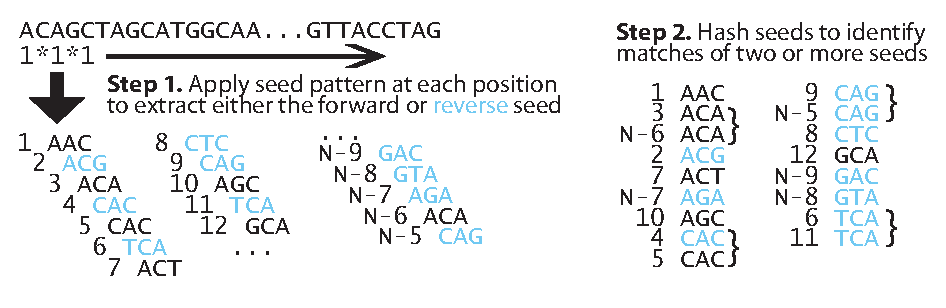
\epsfig{file=string_matching.eps,width=4in}
\caption{Application of the palindromic seed pattern
\texttt{1*1*1} to identify degenerate matching subsequences in a
nucleotide sequence of length $N$. The lexicographically-lesser of
the forward and reverse complement subsequence induced by the seed
pattern is used at each sequence position.}

\label{fig:string_matching}\vspace{-0.2cm}
\end{figure}

Our local multiple alignment filtration method begins by generating
a set of candidate multi-matches using \textit{palindromic} spaced
seed patterns (listed in Table~\ref{table:seedPatterns}). The seed
pattern is evaluated at every position of the input sequence, and
the lexicographically-lesser of the forward and reverse complement
subsequence induced by the seed pattern is hashed to identify seed
matches (Figure~\ref{fig:string_matching}).  The use of
\textit{palindromic} seed patterns offers computational savings by
allowing both strands of DNA to be processed simultaneously.


\begin{table}[h!]
  \centering
\begin{tabular}{|r|r|r|r|r|r|r|r|}
\hline Weight & Pattern &\multicolumn{6}{l|}{Seed Rank by Sequence Identity} \\
\cline{3-8}
&&65\% & 70\% & 75\% & 80\% & 85\% & 90\% \\
\hline\hline

%------------------------------------------------------------------------
5 & \texttt{11*1*11}   & 1 & 1 & 1 & 1 & 1 & 1 \\
%  & \texttt{1**111**1} & 2 & 2 & 2 & 2 & 2 & 7 \\
%  & \texttt{11**1**11} & 3 & 3 & 3 & 3 & 3 & 2 \\
\hline
%-----------------------------------------------------------------------
6 & \texttt{1*11***11*1} & 1 & 1 & 1 & 1 & 1 & 1 \\
% & \texttt{11**1*1**11}  & 2 & 2 & 2 & 2 & 2 & 3 \\
% & \texttt{11*1*1*11}    & 3 & 3 & 3 & 3 & 3 & 1 \\
\hline
%-----------------------------------------------------------------------
7 & \texttt{11**1*1*1**11} & 1 & 1 & 1 & 1 & 1 & 1 \\
% & \texttt{1*11***1***11*1} & 2 & 2 & 2 & 2 & 2 & 2 \\
% & \texttt{11*1***1***1*11} & 3 & 3 & 3 & 3 & 3 & 3 \\
\hline
%-----------------------------------------------------------------------
8 & \texttt{111**1**1**111} & 1 & 1 & 1 & 1 & 1 & 1 \\
% & \texttt{111**1*1**111} & 2 & 2 & 2 & 2 & 2 & 2 \\
% & \texttt{11**1*1*1*1**11} & 4 & 4 & 3 & 4 & 4 & 4 \\
\hline
%-----------------------------------------------------------------------
9 & \texttt{111*1**1**1*111} & 1 & 1 & 1 & 1 & 1 & 1 \\
% & \texttt{111**1**1**1**111} & 3 & 2 & 2 & 2 & 2 & 2 \\
% & \texttt{111**1*1*1**111} & 2 & 3 & 3 & 3 & 3 & 3 \\
\hline
%-----------------------------------------------------------------------
10 & \texttt{111*1**1*1**1*111}  & 1 & 1 & 1 & 1 & 1 & 1 \\
%   & \texttt{111*1**1**1**1*111} & 5 & 3 & 2 & 2 & 2 & 2 \\
%   & \texttt{111*1**11**1*111}   & 2 & 2 & 3 & 3 & 3 & 3 \\
\hline
%--------------------------------------------------------------------------------
11 & \texttt{1111**1*1*1**1111} & 1 & 1 & 1 & 1 & 1 & 2 \\
%   & \texttt{111*1*1**1**1*1*111}   & 3 & 2 & 2 & 2 & 2 & 2 \\
%   & \texttt{111**1**1*1*1**1**111} & 9 & 6 & 3 & 3 & 3 & 3 \\
\hline
%-------------------------------------------------------------------------------
12 & \texttt{1111**1*1*1*1**1111} & 5 & 3 & 1 & 1 & 1 & 1 \\
% & \texttt{1111*1**11**1*1111} & 1 & 1 & 3 & 3 & 2 & 3 \\
% & \texttt{111*11*1***1*11*111} & 3 & 2 & 2 & 2 & 3 & 6 \\
\hline
%-------------------------------------------------------------------------------
13 & \texttt{1111**1**1*1*1**1**1111} & $> 10$ & 5 & 1 & 1 & 1 & 1 \\
% & \texttt{111*1*11**1**11*1*111} & 2 & 1 & 2 & 2 & 2 & 2 \\
% & \texttt{111*1**11*1*11**1*111} & 5 & 3 & 4 & 3 & 4 & 6 \\
\hline
%-------------------------------------------------------------------------------
14 & \texttt{1111**11*1*1*11**1111} & 2 & 2 & 1 & 1 & 1 & 1 \\
% & \texttt{1111*1*11**11*1*1111} & 1 & 1 & 2 & 2 & 2 & 2 \\
% & \texttt{1111*1*1**11**1*1*1111} & 4 & 4 & 3 & 3 & 4 & 5 \\
\hline
%-------------------------------------------------------------------------------
15 & \texttt{1111*1*11**1**11*1*1111} & 1 & 1 & 1 & 1 & 1 & 1 \\
% & \texttt{1111*11**1*1*1**11*1111} & 3 & 2 & 2 & 2 & 3 & 4 \\
% & \texttt{1111**11*1*1*1*11**1111} & 5 & 3 & 3 & 3 & 2 & 2 \\
\hline
%-------------------------------------------------------------------------------
16 & \texttt{1111*1*11**11**11*1*1111} & 2 & 1 & 1 & 1 & 1 & 1 \\
% & \texttt{111*111**1*11*1**111*111} & 5 & 4 & 2 & 2 & 2 & 2 \\
% & \texttt{11111**11*1*1*11**11111} & 4 & 3 & 4 & 3 & 3 & 4 \\
\hline
%-------------------------------------------------------------------------------
18 & \texttt{11111**11*1*11*1*11**11111} & 1 & 1 & 1 & 1 & 1 & 1 \\
% & \texttt{11111*1*11**11**11*1*11111} & 2 & 2 & 2 & 2 & 2 & 2 \\
% & \texttt{1111*11**11*1*1*11**11*1111} & $> 10$ & 6 & 3 & 3 & 3 & 3 \\
\hline
%-----------------------------------------------------------------------
19 & \texttt{1111*111**1*111*1**111*1111} & 5 & 2 & 1 & 1 & 1 & 1 \\
% & \texttt{11111*1*11**111**11*1*11111} & 6 & 4 & 2 & 3 & 4 & 6 \\
% & \texttt{1111*11*111*1*111*11*1111} & 1 & 1 & 4 & 10 & $> 10$ & $> 10$ \\
\hline
%-----------------------------------------------------------------------
20 & \texttt{11111*1*11**11*11**11*1*11111} & $> 10$ & $> 10$ & 3 & 1 & 1 & 1 \\
% & \texttt{11111*11*111**111*11*11111} & 1 & 1 & 8 & $> 10$ & $> 10$ & $> 10$ \\
% & \texttt{11111*1*111**11**111*1*11111} & $> 10$ & $> 10$ & 1 & 2 & 3 & 3 \\
\hline
%-----------------------------------------------------------------------
21 & \texttt{11111*111*11*1*11*111*11111} & 1 & 1 & 1 & 3 & 3 & 2 \\
% & \texttt{111111**11*1*111*1*11**111111} & $> 10$ & 3 & 2 & 1 & 1 & 1 \\
% & \texttt{111111*1*11*111*11*1*111111} & 3 & 2 & 4 & 10 & $> 10$ & 7 \\
\hline

\end{tabular}
\vspace{0.4cm}
  \caption{Palindromic spaced seeds used by \texttt{procrastAligner}.  The sensitivity ranking
  of a seed at various levels of sequence identity is given
  in the columns at right.  A seed with rank 1 is the most sensitive seed pattern for a given weight and
  percent sequence identity. The default seeds used by \texttt{procrastAligner} are
  listed here, while the full list of high-ranking seeds appears on the website.}\label{table:seedPatterns}
\end{table}


\begin{figure}[t]
\centering 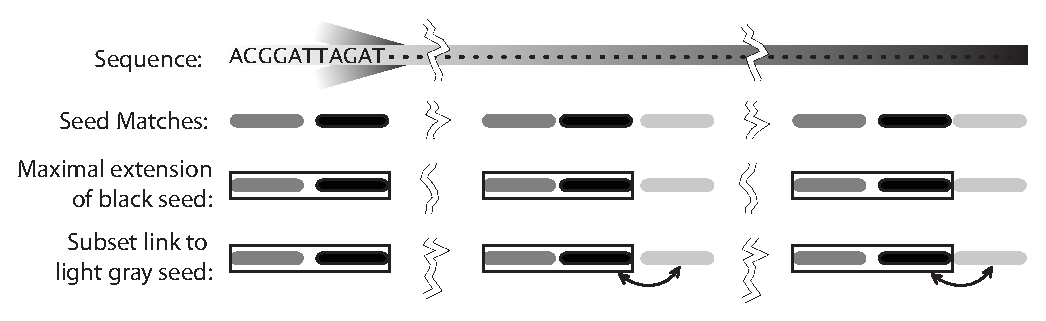
\epsfig{file=simple.eps,width=4in}
\label{fig:simple_extension} \vspace{-0.2cm}\caption{Seed match
extension. Three seed matches are depicted as black, gray, and
light gray regions of the sequence.  Black and gray have
multiplicity 3, while light gray has multiplicity 2.  We maximally
extend the black seed to the left and right and in doing so, the
black seed chains with the gray seed to the left. The light gray
seed is adjacent to only two out of three components in the
extended black seed.  We \textit{procrastinate} and extend the
light gray seed later.  We create a link between light gray and
the extended black seed match.}
\end{figure}

Given an initial set of matching sequence regions, our algorithm
then maximally extends each match to cover the entire surrounding
region of sequence identity.  A visual example of maximal extension
is given by the black match in Figure~\ref{fig:simple_extension}. In
order to extend over each region of sequence $\mathcal{O}(1)$ times,
our method extends matches in order of decreasing multiplicity--we
extend the highest multiplicity matches first. When a match can no
longer be extended without including a gap larger than $w$
characters, our method identifies the neighboring \textit{subset}
matches within $w$ characters, i.e. the light gray seed in
Figure~\ref{fig:simple_extension}. We then \textit{link} each
neighboring subset match to the extended match. We refer to the
extended match as a \textit{superset} match. Rather than immediately
extend the subset match(es), we \textit{procrastinate} and extend
the subset match later when it has the highest multiplicity of any
match waiting to be extended. When extending a match with a linked
superset (light gray in Figure~\ref{fig:simple_extension}), we
immediately include the entire region covered by the linked superset
match--obviating the need to re-examine sequence already covered by
a previous match extension.

\looseness=-1 We score alignments generated by our method using the
entropy equation and exact $p$-value method in~\cite{ref-keich05}.
Our method may produce many hundreds or thousands of local multiple
alignments for a given genome sequence, thus it is important to rank
them by significance.  When computing column entropy, we treat gap
characters as missing data.

\section{Algorithm}

\subsection{Notation and Assumptions}
Given a sequence $\mathcal{S}=s_1, s_2,\dots, s_N$ of length $N$
defined over an alphabet $\{A,C,G,T\}$, our goal is to identify
local multiple alignments on subsequences of $\mathcal{S}$. Our
filtration method first generates candidate chains of ungapped
alignments, which are later scored and possibly re-aligned.  Denote
an ungapped alignment, or match, among subsequences in $\mathcal{S}$
as an object $M$. We assume as input a set of ungapped alignments
$\mathbf{M}$.  We refer the number of regions in $\mathcal{S}$
matched by a given match $M_i \in \mathbf{M}$ as the
\textit{multiplicity} of $M_i$, denoted as $|M_i|$. We refer to each
matching region of $M_i$ as a \textit{component} of $M_i$. Note that
$|M_i| \geq 2~\forall~M \in \mathbf{M}$.  We denote the left-end
coordinates in $\mathcal{S}$ of each component of $M_i$ as $M_i.L_1,
M_i.L_2,\dots, M_i.L_{|M_i|}$, and similarly we denote the right-end
coordinates as $M_i.R_x$.  When aligning DNA sequences, matches may
occur on the forward or reverse complement strands. To account for
this phenomenon we add an orientation value to each matching region:
$M_i.O_x \in \{1,-1\}$, where 1 indicates a forward strand match and
-1 for reverse.

Our algorithm has an important limitation on the matches in
$\mathbf{M}$: no two matches $M_i$ and $M_j$ may have the same
left-end coordinate, e.g. $M_i.L_x \neq M_j.L_y~\forall~i, j, x, y$
except for the identity case when $i=j$ and $x=y$.  This constraint
has been referred to by others as \textit{consistency} and
\textit{transitivity}~\cite{ref-transitivity} of matches.  In the
present work we only require consistency and transitivity of matches
longer than the seed length, e.g. seed matches may overlap.

\subsection{Data structures}
Our algorithm begins with an initialization phase that creates three
data structures. The first data structure is a set of \textit{Match
Records} for each match $M \in \mathbf{M}$.  The \textit{Match
Record} stores $M$, a unique identifier for $M$, and two items which
will be described later in Section~\ref{ssec:extend}: a set of
linked match records, and a \textit{subsuming match pointer}. The
linked match records are further subdivided into four classes: a
left and right \textit{superset link}, and left and right
\textit{subset links}.  The \textit{subsuming match pointer} is
initially set to a \textit{NULL} value. Figure~\ref{fig:proc} shows
a schematic of the match record.

We refer to the second data structure as a \textit{Match Position
Lookup Table}, or $\mathbf{P}$. The table has $N$ entries $p_1,
p_2,\dots,p_N$, one per character of $\mathcal{S}$. The entry for
$p_t$ stores the unique identifier of the match $M_i$ and $x$ for
which $M_i.L_x = t$ or the \textit{NULL} identifier if no match has
$t$ as a left-end coordinate. We call the third data structure a
\textit{Match extension procrastination queue}, or simply the
\textit{procrastination queue}. Again, we denote the multiplicity of
a match $M$ by $|M|$. The \textit{procrastination queue} is a binary
heap of matches ordered on $|M|$ with higher values of $|M|$
appearing near the top of the heap. The heap is initially populated
with all $M \in \mathbf{M}$. This queue dictates the order in which
matches will be considered for extension.


\begin{figure}[t!]
\centering 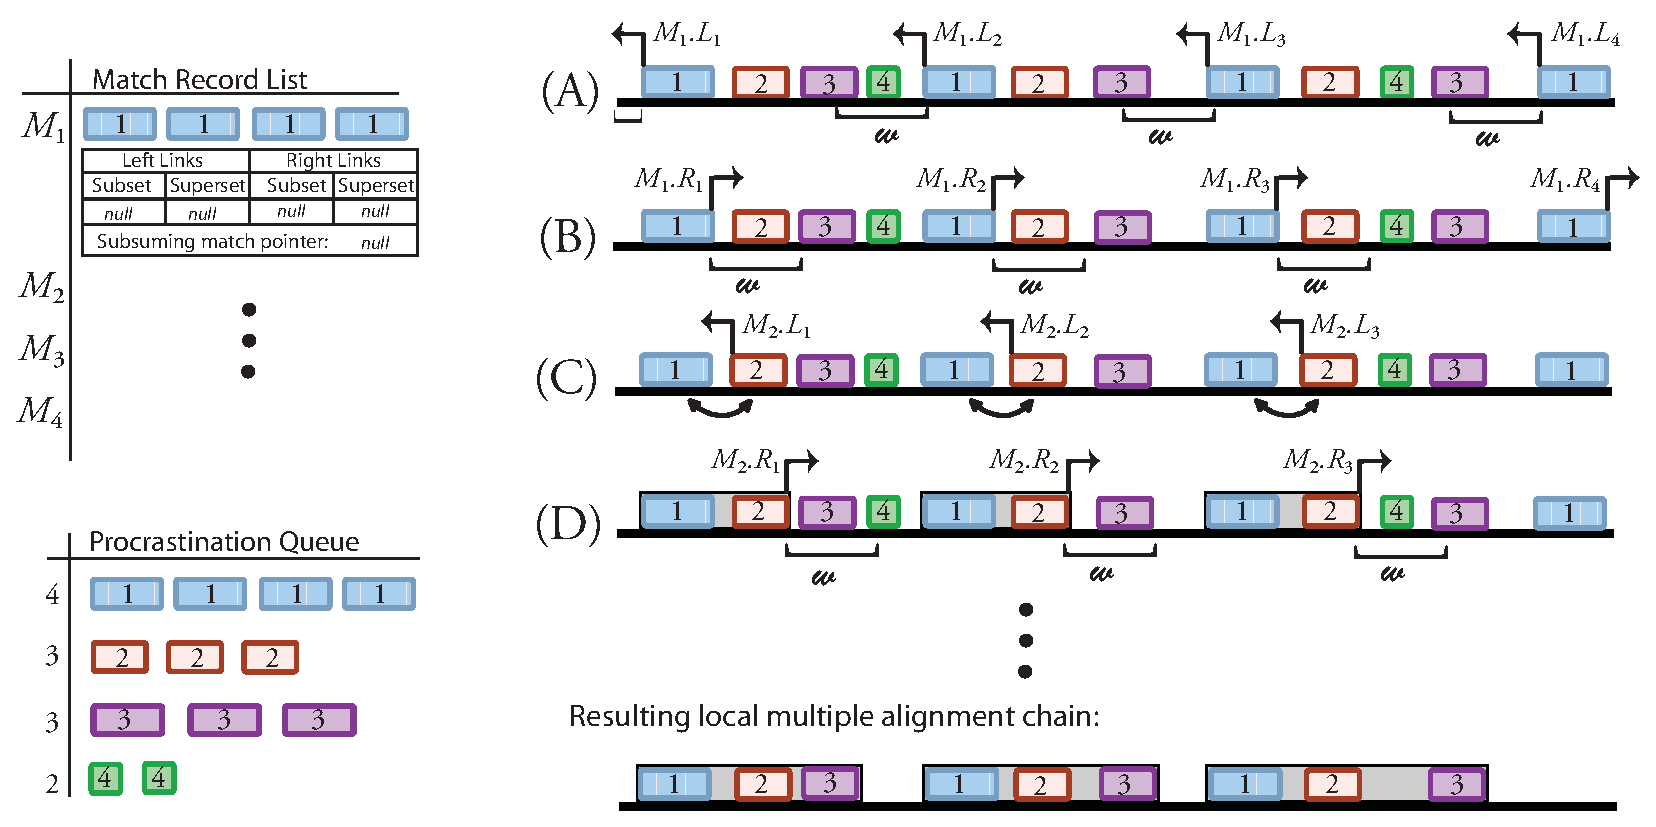
\epsfig{file=proc.eps,width=4.7in} \caption{
\looseness=-1 The match extension process and associated data
structures. \textbf{(A)} First we pop the match at the front of the
procrastination queue: $M_{1}$ and begin its leftward extension.
Starting with the leftmost position of $M_{1}$, we use the
\textit{Match Position Lookup Table} to enumerate every match with a
left-end within some distance $w$. Only $M_4.L_1$ is within $w$ of
$M_1$, so it forms a singleton \textit{neighborhood group} which we
discard. \textbf{(B)} $M_1$ has no \textit{neighborhood groups} to
the left, so we begin extending $M_1$ to the right.  We enumerate
all matches within $w$ to the right of $M_1$. $M_2$ lies to the
right of 3 of 4 components of $M_1$ and so is not subsumed, but
instead gets linked as a right-subset of $M_1$. We add a
left-superset link from $M_{2}$ to $M_1$. \textbf{(C)} Once finished
with $M_{1}$ we pop $M_{2}$ from the front of the procrastination
queue and begin leftward extension. We find the left-superset link
from $M_2$ to $M_1$, so we extend the left-end coordinates of
$M_{2}$ to cover $M_{1}$ accordingly. No further leftward extension
of $M_2$ is possible because $M_1$ has no left-subset links.
\textbf{(D)} Beginning rightward extension on $M_{2}$ we construct a
neighborhood list and find a chainable match $M_{3}$, and a subset
$M_{4}$. We extend $M_2$ to include $M_3$ and mark $M_4$ as
inconsistent and hence not extendable. Upon completion of the
chaining process we have generated a list of local multiple
alignments.} \label{fig:proc}
\end{figure}


\subsection{Extending Matches}\label{ssec:extend}
Armed with the three aforementioned data structures, our algorithm
begins the chaining process with the match at the front of the
\textit{procrastination queue}.  For a match $M_i$ that has not been
subsumed, the algorithm first attempts extension to the left, then
to the right. Extension in each direction is done separately in an
identical manner and we arbitrarily choose to describe leftward
extension first. The first step in leftward match extension for
$M_i$ is to check whether it has a left superset link. If so, we
perform a \textit{link extension} as described later. For extension
of $M_i$ without a superset link, we use the \textit{Match Position
Lookup Table}~$\mathbf{P}$ to enumerate all matches within a fixed
distance $w$ of $M_i$.  For each component $x=1, 2,\dots, |M_i|$ and
distance $d=1, 2,\dots,w$ we evaluate first whether $p_{M_i.L_x-(d
\cdot M_i.O_x)}$ is not \textit{NULL}. If not then $p_{M_i.L_x-(d
\cdot M_i.O_x)}$ stores an entry $\langle M_j, y \rangle$ which is a
pointer to neighboring match $M_j$ and the matching component $y$ of
$M_j$.

In order to consider matches on both forward and reverse strands, we
must evaluate whether $M_i.O_x$ and $M_j.O_y$ are consistent with
each other.  We define the relative orientation of $M_i.O_x$ and
$M_j.O_y$ as $o_{i,j,x,y} = M_i.O_x \cdot M_j.O_y$ which causes
$o_{i,j,x,y} = 1$ if both $M_i.O_x$ and $M_j.O_y$ match the same
strand and $-1$ otherwise. We create a tuple of the form $\langle
M_j, o_{i,j,x,y}, x, d, y \rangle$ and add it to a list called the
\textit{neighborhood list}. In other words, the tuple stores (1) the
unique match ID of the match with a left-end at sequence coordinate
$M_i.L_x-(d \cdot M_i.O_x)$, (2) the relative orientation of
$M_i.O_x$ and $M_j.O_y$, (3) the matching component $x$ of $M_i$,
(4) the distance $d$ between $M_i$ and $M_j$, and (5) the matching
component $y$ of $M_j$. If $M_j=M_i$ for a given value of $d$, we
stop adding \textit{neighborhood list} entries after processing that
one. The \textit{neighborhood list} is then scanned to identify
groups of entries with the same match ID $M_j$ and relative
orientation $o_{i,j,x,y}$. We refer to such groups as
\textit{neighborhood groups}.  Entries in the same
\textit{neighborhood group} that have identical $x$ or $y$ values
are considered ``ties'' and need to be broken. Ties are resolved by
discarding the entry with the larger value of $d$ in the fourth
tuple element: we prefer to chain over shorter distances. After
tiebraking, each \textit{neighborhood group} falls into one of
several categories:

%\begin{enumerate}
\begin{itemize}
\itemsep 0pt

\item\textbf{Superset}: The \textit{neighborhood group} contains
$|M_i|$ separate entries. $M_j$ has higher multiplicity than
$M_i$, e.g. $|M_j|>|M_i|$.  We refer to $M_j$ as a superset of
$M_i$. \item \textbf{Chainable}: The \textit{neighborhood group}
contains $|M_i|$ separate entries. $M_j$ and $M_i$ have equal
multiplicity, e.g. $|M_j|=|M_i|$.  We can chain $M_j$ and $M_i$.
\item \textbf{Subset}:  The \textit{neighborhood group} contains
$|M_j|$ separate entries such that $|M_j| < |M_i|$.  We refer to
$M_j$ as a subset of $M_i$. \item \textbf{Novel Subset}:  The
\textit{neighborhood group} contains $r$ separate entries such
that $r < |M_i| \wedge r < |M_j|$.  We refer to the portion of
$M_j$ in the list as a \textit{novel subset} of $M_i$ and $M_j$
because this combination of matching positions does not exist as a
match in the initial set of matches $\mathbf{M}$.
\end{itemize}
%\end{enumerate}

The algorithm considers each \textit{neighborhood group} for
chaining in the order given above: chainable, subset, and finally,
novel subset.  Superset groups are ignored, as any superset links
would have already been created when processing the superset
match.

\subsubsection{Chainable matches}
To chain match $M_i$ with \textit{chainable} match $M_j$ we first
update the left-end coordinates of $M_i$ by assigning $M_i.L_x
\leftarrow \min(M_i.L_x, M_j.L_y)$ for each $\langle i, j, x,
y\rangle$ in the \textit{neighborhood group} entries. Similarly, we
update the right-end coordinates: $M_i.R_x \leftarrow \max(M_i.R_x,
M_j.R_y)$ for each $\langle i, j, x, y\rangle$ in the group.  If any
of the coordinates in $M_i$ change we make note that a
\textit{chainable} match has been chained. We then update the
\textit{Match Record} for $M_j$ by setting its \textit{subsuming
match pointer} to $M_i$, indicating that $M_j$ is now invalid and is
subsumed by $M_i$. Any references to $M_j$ in the \textit{Match
Position Lookup Table} and elsewhere may be lazily updated to point
to $M_i$ as they are encountered.  If $M_j$ has a left superset
link, the link is inherited by $M_i$ and any remaining neighborhood
groups with \textit{chainable} matches are ignored.
\textit{Chainable} groups are processed in order of increasing $d$
value so that the nearest \textit{chainable} match with a superset
link will be encountered first.  A special case exists when
$M_i=M_j$.  This occurs when $M_i$ represents an inverted repeat
within $w$ nucleotides.  We never allow $M_i$ to chain with itself.

\subsubsection{Subset matches}

We defer subset match processing until no more chainable matches
exist in the neighborhood of $M_i$. A subset match $M_j$ is
considered to be completely contained by $M_i$ when for all $x,y$
pairs in the \textit{neighborhood group}, $M_i.L_x \leq M_j.L_y
\wedge M_j.R_y \leq M_i.R_x$. When subset match $M_j$ is completely
contained by $M_i$, we set the \textit{subsuming match pointer} of
$M_j$ to $M_i$. If the subset match is not contained we create a
\textit{link} from $M_i$ to $M_j$. The subset link is a tuple of the
form $\langle M_i, M_j, x_1, x_2,\dots,x_{|M_j|}\rangle$ where the
variables $x_1 \dots x_{|M_j|}$ are the $x$ values associated with
the $y=1\dots |M_j|$ from the \textit{neighborhood list} group
entries.  The link is added to the left subset links of $M_i$ and we
remove any pre-existing right superset link in $M_j$ and replace it
with the new link.

\subsubsection{Novel subset matches}

A novel subset may only be formed when both $M_i$ and $M_j$ have
already been maximally extended, otherwise we discard any novel
subset matches. When a novel subset exists matches we create a new
match record $M_{novel}$ with left- and right-ends equal to the
outward boundaries of $M_i$ and $M_j$. Rather than extend the novel
subset match immediately, we \textit{procrastinate} and place the
novel subset in the \textit{procrastination queue}. Recall that the
novel subset match contains $r$ matching components of $M_i$ and
$M_j$. In constructing $M_{novel}$, we create links between
$M_{novel}$ and each of $M_i$ and $M_j$ such that $M_{novel}$ is a
left and a right subset of $M_i$ and $M_j$, respectively.  The links
are tuples of the form outlined in the previous section on subset
matches.

Occasionally a \textit{neighborhood group} representing a novel
subset match may have $M_i=M_j$.  This can occur when $M_i$ has
two or more components that form a tandem or overlapping repeat.
If $M_i.L_x$ has $M_i.L_{y}$ in its neighborhood, and $M_i.L_{y}$
has $M_i.L_{z}$ in its neighborhood, then we refer to $\{x,y,z\}$
as a tandem unit of $M_i$.  A given tandem unit contains between
one and $|M_i|$ components of $M_i$, and the set of tandem units
forms a partition on the components of $M_i$. In this situation we
construct a novel subset match record with one component for each
tandem unit of $M_i$.  If $M_i$ has only a single tandem unit then
we continue without creating a novel subset match record.
Figure~\ref{fig:novel} illustrates how we process tandem repeats.


\begin{figure}[t]
\centering 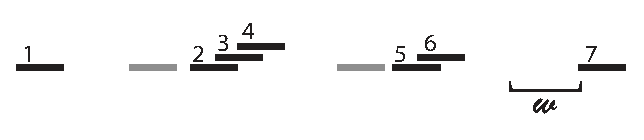
\epsfig{file=novel.eps,width=4.8in,height=0.8in}
\caption{Interplay between tandem repeats and novel subset
matches. There are two initial seed matches, one black, one gray.
The black match has components labelled 1-7, and the neighborhood
size $w$ is shown with respect to component 7. As we attempt
leftward extension of the black match we discover the gray match
in the neighborhood of components 2 and 5 of black. A subset link
is created.  We also discover that some components of the black
match are within each others' neighborhood. We classify the black
match as a tandem repeat and construct a novel subset match with
one component for each of the four tandem repeat units:
$\{1\},\{2,3,4\},\{5,6\},\{7\}$.} \label{fig:novel}
\end{figure}

\subsubsection{After the first round of chaining}

If the \textit{neighborhood list} contained one or more chainable
groups we enter another round of extending $M_i$. The extension
process repeats starting with either \textit{link extension} or by
construction of a new \textit{neighborhood list}. When the
boundaries of $M_i$ no longer change, we classify any subset matches
as either subsumed or outside of $M_i$ and treat them accordingly.
We process novel subsets.  Finally, we may begin extension in the
opposite (rightward) direction. The rightward extension is
accomplished in a similar manner, except that the neighborhood is
constructed from $M_i.R_x$ instead of $M_i.L_x$ and $d$ ranges from
$-1, -2,\dots,-w$ and ties are broken in favor of the largest $d$
value. Where left links were previously used, right links are now
used and vice-versa.

\subsubsection{Chaining the next match}

When the first match popped from the \textit{procrastination queue}
has been maximally extended, we pop the next match from the
\textit{procrastination queue} and consider it for extension. The
process repeats until the \textit{procrastination queue} is empty.
Prior to extending any match removed from the
\textit{procrastination queue}, we check the match's
\textit{subsuming match pointer}.  If the match has been subsumed
extension is unnecessary.

\subsection{Link extension}

To be considered for leftward link extension, $M_i$ must have a left
superset link to another match, $M_j$.  We first extend the
boundaries of $M_i$ to include the region covered by $M_j$ and
unlink $M_i$ from $M_j$.  Then each of the left subset links in
$M_j$ are examined in turn to identify links that $M_i$ may use for
further extension. Recall that the link from $M_i$ to $M_j$ is of
the form $\langle M_j, M_i, x_1, \dots, x_{|M_i|}\rangle$. Likewise,
a left subset link from $M_j$ to another match $M_k$ is of the form
$\langle M_j, M_k, z_1, \dots, z_{|M_k|}\rangle$. To evaluate
whether $M_i$ may follow a given link in the left subsets of $M_j$,
we take the set intersection of the $x$ and $z$ values for each
$M_k$ that is a left subset of $M_j$. We can classify the results of
the set intersection as:

\begin{itemize}
\item \textbf{Superset}:  $\{x_1,\dots,x_{|M_i|}\} \subset \{z_1, \dots, z_{|M_k|}\}$
Here $M_k$ links to every component of $M_j$ that is linked by
$M_i$, in addition to others.
\item \textbf{Chainable}:   $\{x_1,\dots,x_{|M_i|}\} = \{z_1, \dots, z_{|M_k|}\}$
Here $M_k$ links to the same set of components of $M_j$ that $M_i$
links.
\item \textbf{Subset}: $\{x_1,\dots,x_{|M_i|}\} \supset \{z_1, \dots, z_{|M_k|}\}$
Here $M_i$ links to every component of $M_j$ that is linked by
$M_k$, in addition to others.
\item \textbf{Novel Subset}:  $\{x_1,\dots,x_{|M_i|}\} \cap \{z_1, \dots, z_{|M_k|}\} \neq \emptyset$
Here $M_k$ is neither a superset, chainable, nor subset relative to
$M_i$, but the intersection of their components in $M_j$ is
non-empty.  $M_k$ and $M_i$ form a novel subset.
\end{itemize}

Left subset links in $M_j$ are processed in the order given above.
Supersets are never observed, because $M_k$ would have already
unlinked itself from $M_j$ when it was processed (as described
momentarily). When $M_k$ is a chainable match, we extend $M_i$ to
include the region covered by $M_k$ and set the subsuming match
pointer in $M_k$ to point to $M_i$.  We unlink $M_k$ from $M_j$, and
$M_i$ inherits any left superset link that $M_k$ may have.  When
$M_k$ is a subset of $M_i$ we unlink $M_k$ from $M_j$ and add it to
the \textit{deferred subset list} to be processed once $M_i$ has
been fully extended. Finally, we never create novel subset matches
during link extension because $M_k$ will never be a fully extended
match.

If a chainable match was found during leftward link extension, we
continue for another round of leftward extension. If not, we switch
directions and begin rightward extension.

\subsection{Time complexity}
A \textit{neighborhood list} may be constructed at most $w$ times
per character of $\mathcal{S}$, and construction uses sorting by key
comparison, giving $\mathcal{O}(wN \log wN)$ time and space.
Similarly, we spend $\mathcal{O}(wN \log wN)$ time performing link
extension. The upper bound on the total number of components in the
final set of matches is $\mathcal{O}(wN)$. Thus, the overall time
complexity for our filtration algorithm is $\mathcal{O}(wN \log
wN)$.

\section{Results}
We have created a program called \texttt{procrastAligner} for Linux,
Windows, and Mac OS X that implements the described algorithm. Our
open-source implementation is available as C++ source code licensed
under the GPL.

We compare the performance of our method in finding Alu repeats in
the human genome to an Eulerian path method for local multiple
alignment~\cite{ref-related1}. The focus of our algorithm is
efficient filtration, thus we use a scoring metric that evaluates
the filtration sensitivity and specificity of the ungapped alignment
chains produced by our method. We compute sensitivity as the number
of Alu elements hit by a match, out of the total number of Alu
elements.  We compute specificity as the ratio of match components
that hit an Alu to the sum of match multiplicity for all matches
that hit an Alu.  Thus, we do not penalize our method for finding
legitimate repeats that are not in the Alu family.

The comparison between \texttt{procrastAligner} and the Eulerian
method is necessarily indirect, as each method was designed to
solve different (but related) problems.  The Eulerian method uses
a \textit{de Bruijn} graph for filtration, but goes beyond
filtration to compute gapped alignments using banded dynamic
programming. We report scores for a version of the Eulerian method
that computes alignments only on regions identified by its
\textit{de Bruijn} filter. The results suggest that by using our
filtration method, the sensitivity of the Eulerian path local
multiple aligner could be significantly improved.  A second
important distinction is that our method reports \emph{all} local
multiple alignment chains in its allotted runtime, whereas the
Eulerian method identifies only a single alignment.

We also test the ability of our method to provide accurate anchors
for genome alignment.  Using a manually curated alignment of 144
Hepatitis C virus genome sequences~\cite{ref-hcvdb}, we measure the
anchoring sensitivity of our method as the fraction of pairwise
positions aligned in the correct alignment that are also present in
\texttt{procrastAligner} chains.  We measure positive predictive
value as the number of match component pairs that contain correctly
aligned positions out of the total number of match component pairs.
\texttt{procrastAligner} may generate legitimate matches in the
repeat regions of a single genome.  The PPV score penalizes
\texttt{procrastAligner} for identifying such legitimate repeats,
which subsequent genome alignment would have to disambiguate.  Using
a seed size of $9$ and $w=27$, \texttt{procrastAligner} has a
sensitivity of 63\% and PPV of 67\%.
\begin{comment}
Setting the seed size to 7 and $w=45$ increases the sensitivity to
67\% while reducing PPV to 13\%. These scores were calculated on raw
procrastAligner output, without applying a an alignment score
threshold to discard poor alignments. We anticipate that removal of
low-scoring chains will significantly improve PPV.
\end{comment}

\begin{table}[t]
  \centering
\begin{tabular}{lccccccccccc}
\hline Accession & Length & Rep & Family & Alu (bp) & Div, \% & Method & Sn \% & Sp \% & T (s) & Sw & $w$ \\
\hline
\hline AF435921 &  22 Kb &  28 & 10 & 261 (69) & 15.0 (6.4) & Eulerian & 96.3 & 99.4 & 1 & - & - \\
\cline{7-12}                                            &&&&&& procrast & 100 & 95.9 & 1 & 9 & 27 \\
\hline Z15025 &    38 Kb &  52 & 13 & 245 (85) & 15.7 (5.7) & Eulerian & 98.6 & 96.7 & 4 & - & -  \\
\cline{7-12}                                            &&&&&& procrast & 100 & 82.5 & 2 & 9 & 27 \\
\hline AC034110 & 167 Kb &  87 & 18 & 261 (72) & 12.2 (5.9) & Eulerian & 93.5 & 95.2 & 14 & - & - \\
\cline{7-12}                                            &&&&&& procrast & 100 & 97.9 & 3 & 15 & 45 \\
\hline AC010145 & 199 Kb & 118 & 13 & 277 (55) & 15.0 (5.6) & Eulerian & 85.2 & 93.7 & 32 & - & - \\
\cline{7-12}                                            &&&&&& procrast & 99.1 & 99.2 & 3 & 15 & 45 \\
\hline Hs Chr 22 & 1 Mbp & 404 & 32 & 252 (79) & 15.2 (6.1) & Eulerian & 72.4 & 99.4 & 85 & - & - \\
\cline{7-12}                                            &&&&&& procrast & 98.3 & 97.3 & 20 & 15 & 45 \\
\end{tabular}
\vspace{0.1cm}
  \caption{Performance of \texttt{procrastAlign} and the Eulerian path approach on Alu repeats.
  Rep: total number of Alu elements; Family: number of Alu
  families; Alu: average Alu length in bp (S.D.); Div: average Alu divergence (S.D.);
   Sn: sensitivity; Sp: specificity; T: compute time; Sw: palindromic seed weight; $w$: max gap size.  Alus were
  identified by RepeatMasker~\cite{ref-repbase}. We report data for the fast
  version of the Eulerian path method as given by Table~1 of ~\cite{ref-related1}. Sensitivity and specificity
  of \texttt{procrastAlign} was computed as described in the text.}
  \label{table:alu}
\end{table}

\section{ Discussion }

We have described an efficient method for local multiple alignment
filtration.  The chains of ungapped alignments that our filter
outputs may serve as direct input to multiple genome alignment
algorithms. The test results of our prototype implementation on Alu
sequences demonstrate improved sensitivity over \textit{de Bruijn}
filtration.  A promising avenue of further research will be to
couple our filtration method with subsequent refinement using banded
dynamic programming.

The alignment scoring scheme we use can rank alignments by
information content, however a biological interpretation of the
score remains difficult. If a phylogeny and model of evolution for
the sequences were known \textit{a priori} then a biologically
relevant scoring scheme could be used~\cite{ref-tompa05}.
Unfortunately, the phylogenetic relationship for arbitrary local
alignments is rarely known, especially among repetitive elements or
gene families within a single genome and across genomes. It may be
possible to use simulation and MCMC methods to score alignments
where the phylogeny and model of evolution is unknown \textit{a
priori}, but doing so would be computationally prohibitive for our
application.

\section{ Acknowledgements }
AED was supported by NLM Training Grant 5T15LM007359-05. TJT was
supported by Spanish Ministry MECD Grant TIN2004-03382 and AGAUR
Training Grant FI-IQUC-2005. LZ was supported by AFT Grant
146-000-068-112.


\bibliographystyle{splncs}
\small
\bibliography{procrastination}

\begin{comment}
\section{ Appendix: seed patterns }

\begin{table}
  \centering
\begin{tabular}{|c|r|r|r|r|r|r|r|}
\hline Weight & Pattern &\multicolumn{6}{l|} Seed Rank by Sequence Identity \\
\cline{3-8}
&&65\% & 70\% & 75\% & 80\% & 85\% & 90\% \\
\hline\hline

%------------------------------------------------------------------------
5 & \texttt{11*1*11}   & 1 & 1 & 1 & 1 & 1 & 1 \\
  & \texttt{1**111**1} & 2 & 2 & 2 & 2 & 2 & 7 \\
  & \texttt{11**1**11} & 3 & 3 & 3 & 3 & 3 & 2 \\
\hline
%-----------------------------------------------------------------------
6 & \texttt{1*11***11*1} & 1 & 1 & 1 & 1 & 1 & 1 \\
 & \texttt{11**1*1**11}  & 2 & 2 & 2 & 2 & 2 & 3 \\
 & \texttt{11*1*1*11}    & 3 & 3 & 3 & 3 & 3 & 1 \\
\hline
%-----------------------------------------------------------------------
7 & \texttt{11**1*1*1**11} & 1 & 1 & 1 & 1 & 1 & 1 \\
 & \texttt{1*11***1***11*1} & 2 & 2 & 2 & 2 & 2 & 2 \\
 & \texttt{11*1***1***1*11} & 3 & 3 & 3 & 3 & 3 & 3 \\
\hline
%-----------------------------------------------------------------------
8 & \texttt{111**1**1**111} & 1 & 1 & 1 & 1 & 1 & 1 \\
 & \texttt{111**1*1**111} & 2 & 2 & 2 & 2 & 2 & 2 \\
 & \texttt{11**1*1*1*1**11} & 4 & 4 & 3 & 4 & 4 & 4 \\
\hline
%-----------------------------------------------------------------------
9 & \texttt{111*1**1**1*111} & 1 & 1 & 1 & 1 & 1 & 1 \\
 & \texttt{111**1**1**1**111} & 3 & 2 & 2 & 2 & 2 & 2 \\
 & \texttt{111**1*1*1**111} & 2 & 3 & 3 & 3 & 3 & 3 \\
\hline
%-----------------------------------------------------------------------
10 & \texttt{111*1**1*1**1*111}  & 1 & 1 & 1 & 1 & 1 & 1 \\
   & \texttt{111*1**1**1**1*111} & 5 & 3 & 2 & 2 & 2 & 2 \\
   & \texttt{111*1**11**1*111}   & 2 & 2 & 3 & 3 & 3 & 3 \\
\hline
%--------------------------------------------------------------------------------
11 & \texttt{1111**1*1*1**1111} & 1 & 1 & 1 & 1 & 1 & 2 \\
   & \texttt{111*1*1**1**1*1*111}   & 3 & 2 & 2 & 2 & 2 & 2 \\
   & \texttt{111**1**1*1*1**1**111} & 9 & 6 & 3 & 3 & 3 & 3 \\
\hline
%-------------------------------------------------------------------------------
12 & \texttt{1111**1*1*1*1**1111} & 5 & 3 & 1 & 1 & 1 & 1 \\
 & \texttt{1111*1**11**1*1111} & 1 & 1 & 3 & 3 & 2 & 3 \\
 & \texttt{111*11*1***1*11*111} & 3 & 2 & 2 & 2 & 3 & 6 \\
\hline
%-------------------------------------------------------------------------------
13 & \texttt{1111**1**1*1*1**1**1111} & $> 10$ & 5 & 1 & 1 & 1 & 1 \\
 & \texttt{111*1*11**1**11*1*111} & 2 & 1 & 2 & 2 & 2 & 2 \\
 & \texttt{111*1**11*1*11**1*111} & 5 & 3 & 4 & 3 & 4 & 6 \\
\hline
%-------------------------------------------------------------------------------
14 & \texttt{1111**11*1*1*11**1111} & 2 & 2 & 1 & 1 & 1 & 1 \\
 & \texttt{1111*1*11**11*1*1111} & 1 & 1 & 2 & 2 & 2 & 2 \\
 & \texttt{1111*1*1**11**1*1*1111} & 4 & 4 & 3 & 3 & 4 & 5 \\
\hline
%-------------------------------------------------------------------------------
15 & \texttt{1111*1*11**1**11*1*1111} & 1 & 1 & 1 & 1 & 1 & 1 \\
 & \texttt{1111*11**1*1*1**11*1111} & 3 & 2 & 2 & 2 & 3 & 4 \\
 & \texttt{1111**11*1*1*1*11**1111} & 5 & 3 & 3 & 3 & 2 & 2 \\
\hline
%-------------------------------------------------------------------------------
16 & \texttt{1111*1*11**11**11*1*1111} & 2 & 1 & 1 & 1 & 1 & 1 \\
 & \texttt{111*111**1*11*1**111*111} & 5 & 4 & 2 & 2 & 2 & 2 \\
 & \texttt{11111**11*1*1*11**11111} & 4 & 3 & 4 & 3 & 3 & 4 \\
\hline
%-------------------------------------------------------------------------------
18 & \texttt{11111**11*1*11*1*11**11111} & 1 & 1 & 1 & 1 & 1 & 1 \\
 & \texttt{11111*1*11**11**11*1*11111} & 2 & 2 & 2 & 2 & 2 & 2 \\
 & \texttt{1111*11**11*1*1*11**11*1111} & $> 10$ & 6 & 3 & 3 & 3 & 3 \\
\hline
%-----------------------------------------------------------------------
19 & \texttt{1111*111**1*111*1**111*1111} & 5 & 2 & 1 & 1 & 1 & 1 \\
 & \texttt{11111*1*11**111**11*1*11111} & 6 & 4 & 2 & 3 & 4 & 6 \\
 & \texttt{1111*11*111*1*111*11*1111} & 1 & 1 & 4 & 10 & $> 10$ & $> 10$ \\
\hline
%-----------------------------------------------------------------------
20 & \texttt{11111*1*11**11*11**11*1*11111} & $> 10$ & $> 10$ & 3 & 1 & 1 & 1 \\
 & \texttt{11111*11*111**111*11*11111} & 1 & 1 & 8 & $> 10$ & $> 10$ & $> 10$ \\
 & \texttt{11111*1*111**11**111*1*11111} & $> 10$ & $> 10$ & 1 & 2 & 3 & 3 \\
\hline
%-----------------------------------------------------------------------
21 & \texttt{11111*111*11*1*11*111*11111} & 1 & 1 & 1 & 3 & 3 & 2 \\
 & \texttt{111111**11*1*111*1*11**111111} & $> 10$ & 3 & 2 & 1 & 1 & 1 \\
 & \texttt{111111*1*11*111*11*1*111111} & 3 & 2 & 4 & 10 & $> 10$ & 7 \\
\hline
\end{tabular}
\vspace{0.2cm}
  \caption{Palindromic spaced seeds used by \texttt{procrastAligner}.  The sensitivity ranking
  of a seed at various levels of sequence identity is given
  in the columns at right.  A seed with rank 1 is the most sensitive seed pattern for a given weight and
  percent sequence identity. The
  first listed seed of a given weight is used by default unless otherwise specified
  by the user.}\label{table:seedPatternsFull}
\end{table}
\end{comment}
\end{document}
